\documentclass{article}
\usepackage[margin=1in]{geometry}
\usepackage{pgf}
\usepackage{tikz}
\usetikzlibrary{arrows,automata}
\usepackage[latin1]{inputenc}
\usepackage{listings}
\lstdefinestyle{customc}{
  belowcaptionskip=1\baselineskip,
  breaklines=true,
  frame=L,
  xleftmargin=\parindent,
  language=C,
  showstringspaces=false,
  basicstyle=\footnotesize\ttfamily,
  keywordstyle=\bfseries\color{green!40!black},
  commentstyle=\itshape\color{purple!40!black},
  identifierstyle=\color{blue},
  stringstyle=\color{orange},
}
\lstset{escapechar=@,style=customc}
\begin{document}
\lstinputlisting[caption=page\_check\_references, style=customc]{src/page_check_references.c}
\begin{figure}
\begin{center}
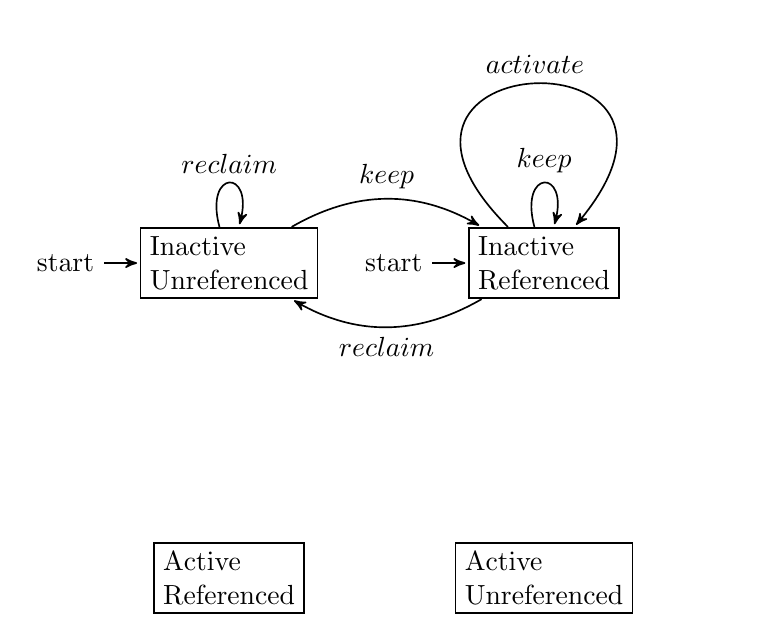
\begin{tikzpicture}[->,>=stealth',shorten >=1pt,auto,node distance=4cm,
                    semithick]

  \tikzstyle{every state}=[rectangle,draw,align=left]

  \node[initial,state] (IU)               {Inactive \\ Unreferenced};
  \node[initial,state] (IR) [right of=IU] {Inactive \\ Referenced};
  \node[state] (AU) [below of=IR] {Active \\ Unreferenced};
  \node[state] (AR) [below of=IU] {Active \\ Referenced};

  \path
  (IU) edge [loop above]                 node {$reclaim$}   (IU)
  (IU) edge [bend  left]                 node {$keep$}            (IR)
  (IR) edge [bend  left]                 node {$reclaim$} (IU)
  (IR) edge [loop above]                 node {$keep$}            (IR)
  (IR) edge [out=135,in=50,looseness=10] node {$activate$}      (IR);
\end{tikzpicture}
\end{center}
\caption{Simplified Automata}
\end{figure}
\begin{figure}
\begin{center}
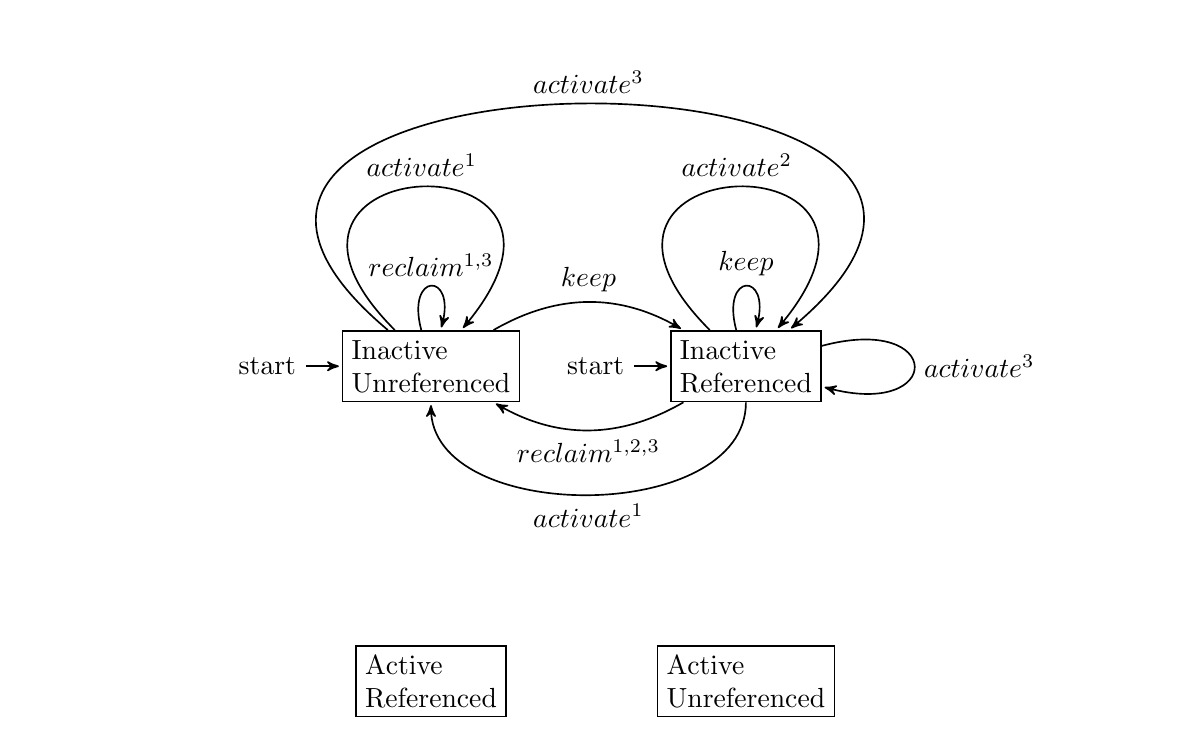
\begin{tikzpicture}[->,>=stealth',shorten >=1pt,auto,node distance=4cm,
                    semithick]

  \tikzstyle{every state}=[rectangle,draw,align=left]

  \node[initial,state] (IU)               {Inactive \\ Unreferenced};
  \node[initial,state] (IR) [right of=IU] {Inactive \\ Referenced};
  \node[state] (AU) [below of=IR] {Active \\ Unreferenced};
  \node[state] (AR) [below of=IU] {Active \\ Referenced};

  \path
  (IU) edge [loop above]                 node {$reclaim^{1,3}$}   (IU)
  (IU) edge [bend  left]                 node {$keep$}            (IR)
  (IU) edge [out=140,in=40,looseness=03] node {$activate^3$}      (IR)
  (IU) edge [out=135,in=50,looseness=10] node {$activate^1$}      (IU)
  (IR) edge [bend  left=90]              node {$activate^1$}      (IU)
  (IR) edge [bend  left]                 node {$reclaim^{1,2,3}$} (IU)
  (IR) edge [loop above]                 node {$keep$}            (IR)
  (IR) edge [out=135,in=50,looseness=10] node {$activate^2$}      (IR)
  (IR) edge [loop right]                 node {$activate^3$}      (IR);
\end{tikzpicture}
\end{center}
\caption{Automata}
\end{figure}
\begin{table}
\begin{tabular}{|l|l|}
\hline
Transition & Condition \\
\hline
$reclaim^1$  page & $VM\_LOCKED$                                     \\
$activate^1$ page & PageSwapBacked(page)                             \\
$activate^2$ page & $referenced\_ptes > 1$                           \\
$activate^3$ page & $VM\_EXEC$                                       \\
$keep$       page & $referenced\_ptes > 0$                           \\
$reclaim^2$  page & $referenced\_ptes = 0$ And !PageSwapBacked(page) \\
$reclaim^3$  page & $referenced\_ptes = 0$                           \\
\hline
Condition               & Note \\
\hline
$referenced\_ptes = 0$ & the page was not accessed through virtual memory addressing. \\
$referenced\_ptes > 0$ & a page table entry access bit was set. \\
$referenced\_ptes > 1$ & the page is shared and multiple access bits were set. \\
\hline

\end{tabular}
\caption{Legend}
\end{table}
\end{document}